\sh reduces each molecule of a dataset to its scaffold and arrange the resulting scaffolds hierarchically in a tree structure called \textit{Scaffold Tree}.
Scaffold Trees were first described by \cite{schuffenhauer_et_al2007} and allow navigation through the molecules in a meaningful manner.
In this chapter you will learn how to generate a scaffold tree.


\begin{figure}[!htb]
   \centering
   \subfloat[][Scaffold Tree Generation Dialog] {
      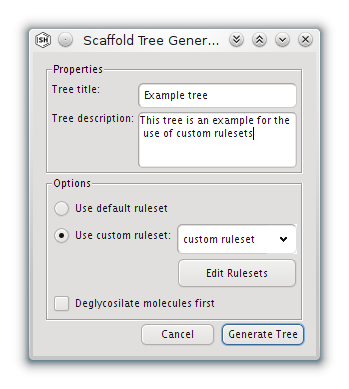
\includegraphics[width=0.45\textwidth]{images/sh_tree_generation_dialog.png}
      \label{fig:treegeneration:generationoptions}
   }
   \quad
   \subfloat[][Tree Generation Progress] {
      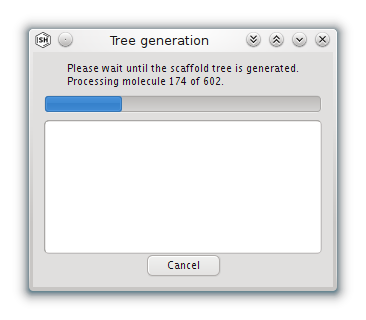
\includegraphics[width=0.45\textwidth]{images/sh_tree_generation_progress_dialog.png}
      \label{fig:treegeneration:progress}
   }
   \caption[Scaffold Tree Generation Dialog / Tree Generation Process Window]{Dialog \protect\subref{fig:treegeneration:generationoptions} allows you to configure tree generation; \protect\subref{fig:treegeneration:progress} shows the dialog indicating the process during tree generation}
   \label{fig:treegeneration}
\end{figure}


Fig. \ref{fig:treegeneration:generationoptions} shows the \guidialog{Scaffold Tree Generation Dialog}, where you have to fill in a tree title,
can fill in an explaining description of the tree and have to choose some generation options.
See \subsecref{subsec:scaffoldhunter:customrules} and \subsecref{subsec:scaffoldhunter:deglycosylate} to learn more about the options you have.
By clicking \gui{Cancel}, you will be returned to the \secref{sec:scaffoldhunter:datasetmanagement} dialog.
By clicking \gui{Generate Tree} \sh will generate and store the tree with the given options,
while showing the progress in a window shown in Fig. \ref{fig:treegeneration:progress}.
	
\subsubsection{Using Custom Rules} \label{subsec:scaffoldhunter:customrules}
The ring pruning rules define an order according to which rings are pruned from the scaffold for the generation of the scaffold tree. In 
each step of the tree generation, starting from a child scaffold, all possible parent scaffolds are generated that could be obtained by 
the removal of one peripheral ring. The hierarchical set of rules is used to select one pruning among the candidates, i.e. one ring to be 
pruned. Thereby each rule might decrease the number of candidate prunings until only a single solutions remains. In the default mode the 
rules are applied exactly as described in the Scaffold Tree publication~\cite{schuffenhauer_et_al2007}. 
To provide more flexibility with ring pruning, the custom rules option allows to define a customized subset of rules in a desired order 
selected from a wider range of implemented rules. 
For this purpose a generic framework for rules was defined. Each rule consists of two parts:

\begin{enumerate}
 \item a numerical descriptor that describes either each of the potentially pruned rings or each of the different remaining parent 
scaffolds that could be generated from the child scaffold, and 
 \item a selection criterion that defines whether the candidate prunings with the minimum or the maximum descriptor value should be 
retained (i.e. each pruning candidate except the minimum / maximum are removed from the set of remaining pruning operations) and passed 
on to the next rule until only one pruning remains.
\end{enumerate}

If multiple solutions have the minimum / maximum rule descriptor value, all of these are retained. If all pruning candidates of a 
scaffold result in the same descriptor value, all pruning candidates are passed on to the next rule.
Like with in the original ruleset, if the custom rules are not successful to identify a single pruning, a tie-break rule is evoked that 
selects the first scaffolds after lexicographically sorting the parent scaffolds according to their canonical SMILES strings.\\

To choose a set of rules for tree generation, select a ruleset from the drop-down box in the \guidialog{Scaffold Tree Generation Dialog} shown on Fig. \ref{fig:treegeneration:generationoptions}.
If no appropriate ruleset exists, you first have to click on \gui{Edit Rulesets} to open the \guidialog{Ruleset Management Dialog} and create a custom ruleset.\\

\begin{figure}[ht]
   \centering
   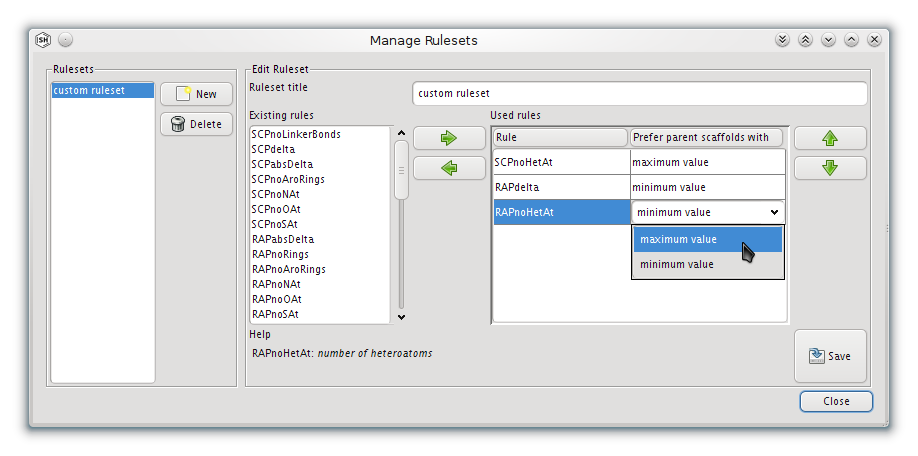
\includegraphics[width=\textwidth]{images/sh_manage_rulesets_dialog.png}
   \caption{Ruleset Management Dialog}
   \label{fig:ruleset_management}
\end{figure}

On the left side of \figref{fig:ruleset_management} you see a list of currently available rulesets.
If no ruleset is available you can create a new one by clicking \gui{New Ruleset}.

If you select a ruleset from the ruleset list, then you can edit the ruleset with the controls located on the right side of the dialog.
You have to enter a name for the ruleset and you can choose rules from the existing ruleset list on the left side of the dialog to be used in your custom ruleset.
To use a rule, select it and move it to the used rule list by clicking on the right arrow button.
You can even select and move multiple rules by using the \texttt{Shift} or \texttt{Ctrl} modifier keys during selection.\\

Each row in the used rule list represents one rule, with the descriptor name in the first column, and the selection criterion in the second column.
To change the selection criterion of a rule, select "maximum value" or "minimum value" from the corresponding drop-down box.\\

The order of the rules in the used rules list determines the order of execution of the rules.
You can change the execution order of a rule by selecting it first and then clicking on the arrow buttons to move it up or down.

If you finished editing your custom ruleset, click the \gui{Save} button to save the ruleset.\\

An adaption of the default rules within this framework would look like (for detailed explanation of the rule name see below):

\begin{verbatim}
RRPsize11p "minimum value"
SCPnoLinkerBonds "minimum value"	
SCPabsDelta "maximum value"	
SCPdelta "maximum value"
RRPsize6 "maximum value"	
RRPsize5 "maximum value"	
RRPsize3 "maximum value"	
RRPnoHetAt "minimum value"	
RRPnoNAt "minimum value"	
RRPnoOAt "minimum value"	
RRPnoSAt "minimum value"	
RRPringSize "minimum value"	
SCPnoAroRings "minimum value"	
RRPhetAtLinked "maximum value"
\end{verbatim}

\paragraph*{Implemented Rule Descriptors}
Three classes of descriptors are provided:

\begin{tabular}{lp{.5\textwidth}}
\texttt{SCP} (SCaffold Properties)       & properties of the resulting parent scaffold after pruning \\
\texttt{RAP} (Ring Assembly Properties)  & properties of the ring assembly containing the ring to be pruned \\
\texttt{RRP} (Removed Ring Properties)   & properties of the ring to be pruned \\
\end{tabular}

\paragraph*{Detailed Description of the Properties}
The names on the left are the rules that can be used in a ruleset.

\begin{longtable}{lp{0.6\textwidth}}
\textbf{Rule}			& \textbf{Description} \\
\toprule
\texttt{SCPnoLinkerBonds}	& number of acyclic linker bonds \\
\texttt{SCPdelta}		& delta value indicating nonlinear ring fusions, spiro systems bridged systems as defined in \cite{schuffenhauer_et_al2007} \\
\texttt{SCPabsDelta}		& absolute delta value indicating nonlinear ring fusions, spiro systems bridged systems as defined in \cite{schuffenhauer_et_al2007} \\
\texttt{SCPnoAroRings}		& number of aromatic rings \\
\texttt{SCPnoHetAt}		& number of heteroatoms \\
\texttt{SCPnoNAt}		& number of nitrogen atoms \\
\texttt{SCPnoOAt}		& number of oxygen atoms \\
\texttt{SCPnoSAt}		& number of sulfur atoms \\
\midrule
\texttt{RAPdelta}		& delta value \\
\texttt{RAPabsDelta}		& absolute delta value \\
\texttt{RAPnoRings}		& number of rings \\
\texttt{RAPnoAroRings}		& number of aromatic rings \\
\texttt{RAPnoHetAt}		& number of heteroatoms \\
\texttt{RAPnoNAt}		& number of nitrogen atoms \\
\texttt{RAPnoOAt}		& number of oxygen atoms \\
\texttt{RAPnoSAt}		& number of sulfur atoms \\
\midrule
\texttt{RRPringSize}		& size of removed ring \\
\texttt{RRPnoHetAt}		& number of heteroatoms \\
\texttt{RRPnoNAt}		& number of nitrogen atoms \\
\texttt{RRPnoOAt}		& number of oxygen atoms \\
\texttt{RRPnoSAt}		& number of sulfur atoms \\
\texttt{RRPhetAtLinked}		& binary descriptor (``maximum value'' = \texttt{True}, ``minimum value'' = \texttt{False}) indicating whether removed ring was linked via a linker to a heteroatom in a ring \\
\texttt{RRPsize3}		& binary descriptor: removed ring of size 3 \\
\texttt{RRPsize4}		& binary descriptor: removed ring of size 4 \\
\texttt{RRPsize5}		& binary descriptor: removed ring of size 5 \\
\texttt{RRPsize6}		& binary descriptor: removed ring of size 6 \\
\texttt{RRPsize7}		& binary descriptor: removed ring of size 7 \\
\texttt{RRPsize8}		& binary descriptor: removed ring of size 8 \\
\texttt{RRPsize9}		& binary descriptor: removed ring of size 9 \\
\texttt{RRPsize10}		& binary descriptor: removed ring of size 10 \\
\texttt{RRPsize11}		& binary descriptor: removed ring of size 11 \\
\texttt{RRPsize11p}		& binary descriptor: removed ring of size more than 11 \\
\texttt{RRPlinkerLen1}		& binary descriptor: removed ring connected via linker of length 1 \\
\texttt{RRPlinkerLen2}		& binary descriptor: removed ring connected via linker of length 2 \\
\texttt{RRPlinkerLen3}		& binary descriptor: removed ring connected via linker of length 3 \\
\texttt{RRPlinkerLen4}		& binary descriptor: removed ring connected via linker of length 4 \\
\texttt{RRPlinkerLen5}		& binary descriptor: removed ring connected via linker of length 5 \\
\texttt{RRPlinkerLen6}		& binary descriptor: removed ring connected via linker of length 6 \\
\texttt{RRPlinkerLen7}		& binary descriptor: removed ring connected via linker of length 7 \\
\texttt{RRPlinkerLen7p}		& binary descriptor: removed ring connected via linker of length more than 7 \\
\bottomrule
\caption{Rule descriptors}
\end{longtable}

\subsubsection{Deglycosylate Molecules First} \label{subsec:scaffoldhunter:deglycosylate}
This check box activates the deglycosylation of molecules that was described in \cite{Koch2005}. 
The procedure iteratively removes terminal pentose and hexose sugars based on a substructure matching before generation of the scaffold 
tree. It is especially useful when processing natural product structures, i.e. from the Dictionary of Natural Products (DNP), that 
contain molecules with multiple glycosylation patterns.
